\chapter{Earth System Data Middleware}

\section{Introduction}

\tab
The Earth System Data Middleware (ESDM) has been designed to deal with the fact that existing data libraries for standardised data description and optimised I/O, such as NetCDF, HDF5 and GRIB, do not have suitable performance-portable optimisations for large-scale simulation workflows in climate and weather.

This text provides an overview of the developed prototype for ESDM. From the application perspective, ESDM provides a data model that manages datasets in virtual containers with their metadata. Datasets are partitioned into fragments, that are stored via various data backends. The middleware operates these data autonomously, i.e., decides on the storage backend and exposes characterisations of the data centres, that are then used by backend plugins to perform the fitting segmentation and distribution of data to storage objects and fragments.

The developed prototype, which has a refined architecture design from the previous Deliverable (D4.2), implements the following key features:

\begin{itemize}

\item provides relaxed access semantics, tailored to scientific data generation for independent writes;

\item yields better performance via optimised data layout schemes;

\item understands application data structures and scientific metadata;

\item maps data structures flexibly to multiple storage backends with different performance characteristics based on site-specific configuration;

\item separates file metadata operations from data access, which enables the exploitation of acceleration techniques. With traditional NetCDF and GRIB data, the relevant application metadata and much of the information about actual data layout is invisible to the file system (whether parallel or serial); and

\item integrates with the NetCDF API as a subcomponent which allows applications to replace the standard NetCDF library with the ESDM supported library. By utilising standard tools belonging to the ESDM library, import/export files application between ESDM and NetCDF are now possible.

\end{itemize}

The significant benefit of the ESDM design is that it provides the opportunity of a rich variety of future features without user intervention.

\section{Logical View: Data Model}
\label{sec: viewpoints/logical/data model}

\tab
The data model of a system organises elements of data, standardises how they represent data entities and how users can interact with the data.
The data model can be split into three layers:

\begin{description}

\item[The Conceptual Data Model]

\tab

\Cref{subsec: conceptual data model} describes the entities and the semantics of the domain represented by the data model and the typical operations to manipulate the data.
In our case, the scientific domain is NWP/Climate.

\item[The Logical Data Model]

\tab

\Cref{subsec-ldm} describes the abstraction level provided by the system, how the domain entities are mapped to objects provided by the system\footnote{An entity of the domain model such as a car could be assigned to one or several objects.}, and the supported operations for accessing and manipulating these objects.
In short, the logical data model defines the semantics when using the operations to access and manipulate the system objects.
For example, a system object of a relational model is a table -- representing attributes of a set of objects -- and a row of a table represents attributes of a single object.

\item[The Physical Data Model]

\tab

\Cref{chap:components and backends} describes how the logical entities are finally mapped to objects/files/regions on the available hardware.
The backends of ESDM partly cover the physical data model, and the descriptions will stop at this level of abstraction.

\end{description}

\subsection{Conceptual Data Model}
\label{subsec: conceptual data model}

\tab
Our conceptual data model is aligned with the needs of domain scientists from climate and weather. It reuses and extends the concepts introduced for a data model proposed by the Climate and Forecasting conventions for NetCDF data\footnote{``A CF Data Model and Implementation'', Hassel et al., 2017, GMD submitted.}.
This scientific data model consists of the following key entities:

\begin{description}

\item[Variable]

A variable, $V$, defines a set of data representing a discrete (generally scalar) quantity within a sampling domain, $d$.  Whatever the sampling regime and dimensionality, values of a variable $V$ will be laid out in storage. $V$ is accompanied by

\item[Metadata]

Metadata includes, at the minimum, a name (e.g. height, time), but may also include units and information about dimensionality, directionality, among others (e.g. degrees, months, days-since-a-particular-time-using-a-particular-calendar). This information may be inserted directly, e.g. via a (key, value) pair such as that necessary to expose $z=1.5m$ for the air temperature at $1.5m$, or indirectly, e.g. via pointers to other generic coordinate variables which describe the sampled domain. Additionally, there may be a dictionary of supporting metadata which may or may not conform to an external semantic convention or standard. Such metadata could include information about the tool used to observe or simulate the specific variable.  Additional metadata is also required for all the other entities described below.

\item[Dimension]

The sampling domain $d$ is defined by the dimensions, which also represents the coordinate axis. Dimensions will include metadata or details of how to construct an algorithm to find the exact sampling coordinates, perhaps using a well-known algorithm such as an ISO 8601 time.

\item[Coordinate]

Coordinates are the set of values at which data is sampled along any given dimension. They may be
explicitly defined by indexing into a coordinate variable, or implicitly determined by an algorithm. When we talk about coordinates, it is usually clear if we mean the $N$-dimensional coordinate to address data in a given variable or if we mean the coordinate along one dimension.

\item[Cell]

The data values are known as points, which may or may not represent a cell. Cells are $N$-dimensional shapes where the dimensionality may or may not fully encompass the dimensionality of the domain.
$N$-dimensional shapes can be implicitly defined as the Cartesian product of all dimensional coordinates forming the data cube of the cell. They can also be explicitly defined, either by providing bounds on the coordinate variables (via metadata) or by introducing a new variable which expressly represents the functional boundaries of the cell (as might happen in a finite element unstructured grid).

\item[Data Set]

Variables can be aggregated into data sets. A data set contains multiple variables that logically belong together, and should be associated with metadata describing the reason for the aggregation.  Variables must have unique names within a data set. Our conceptual model assumes that all variables are scalars, but clearly, the use of these scalars requires more complex interpretation.

\item[Data Type]

The data type defines the types of values that are valid and the operations that can be conducted.
While we are mostly dealing with scalars, they may not be amenable to interpretation as real numbers.
For example, a variable may be storing an integer which points into a taxonomy of categories of land-surface-types.
More complex structures could include complex data types such as vectors, compressed ensemble values, or structures within this system with their interpretation being handled outside of ESDM and documented in metadata. This feature allows ESDM to limit itself to simple data types plus arbitrary length blocks of bits.

\item[Operators]

An operator defines the possible manipulations on the conceptual entities. The most straightforward operators will include \texttt{create}, \texttt{read}, \texttt{update} and \texttt{delete} applied to an entity as a whole, or a subset. However, even these simple operators will come with constraints. For example, it should not be possible to delete a coordinate variable without deleting the parent variable as well. There has to be a separation of concerns between operators which can be handled within the ESDM subsystem and those requiring external logic. Operators that require external logic include subsetting. ESDM will support simple subsetting using simple coordinates, but complex subsets, such as finding a region in real space from dimensions spanned using an algorithm or coordinate variable, may require knowledge of how such algorithms or variables are specified.
Such knowledge is embedded in conventions such as the CF NetCDF convention, and this knowledge could only be provided to ESDM via appropriate operator plugins.

\end{description}

\subsection{Logical Data Model}
\label{subsec-ldm}

\tab
The logical data model describes how data is represented inside ESDM, the operations to interact with the data and their semantics. There are four first-class entities in the ESDM logical data model: \textbf{variable}s, \textbf{fragment}s, \textbf{container}s, and \textbf{metadata}. ESDM \textbf{reference}s may link ESDM entities, and a key property which emerges from the use of references is that an ESDM entity instance may not be deleted while references to it still exist. The use of reference counting will ensure this property as well as avoid dangling pointers. \Cref{fig:data-model} gives an overview of the logical data model.

\begin{figure}[H]
    \centering
    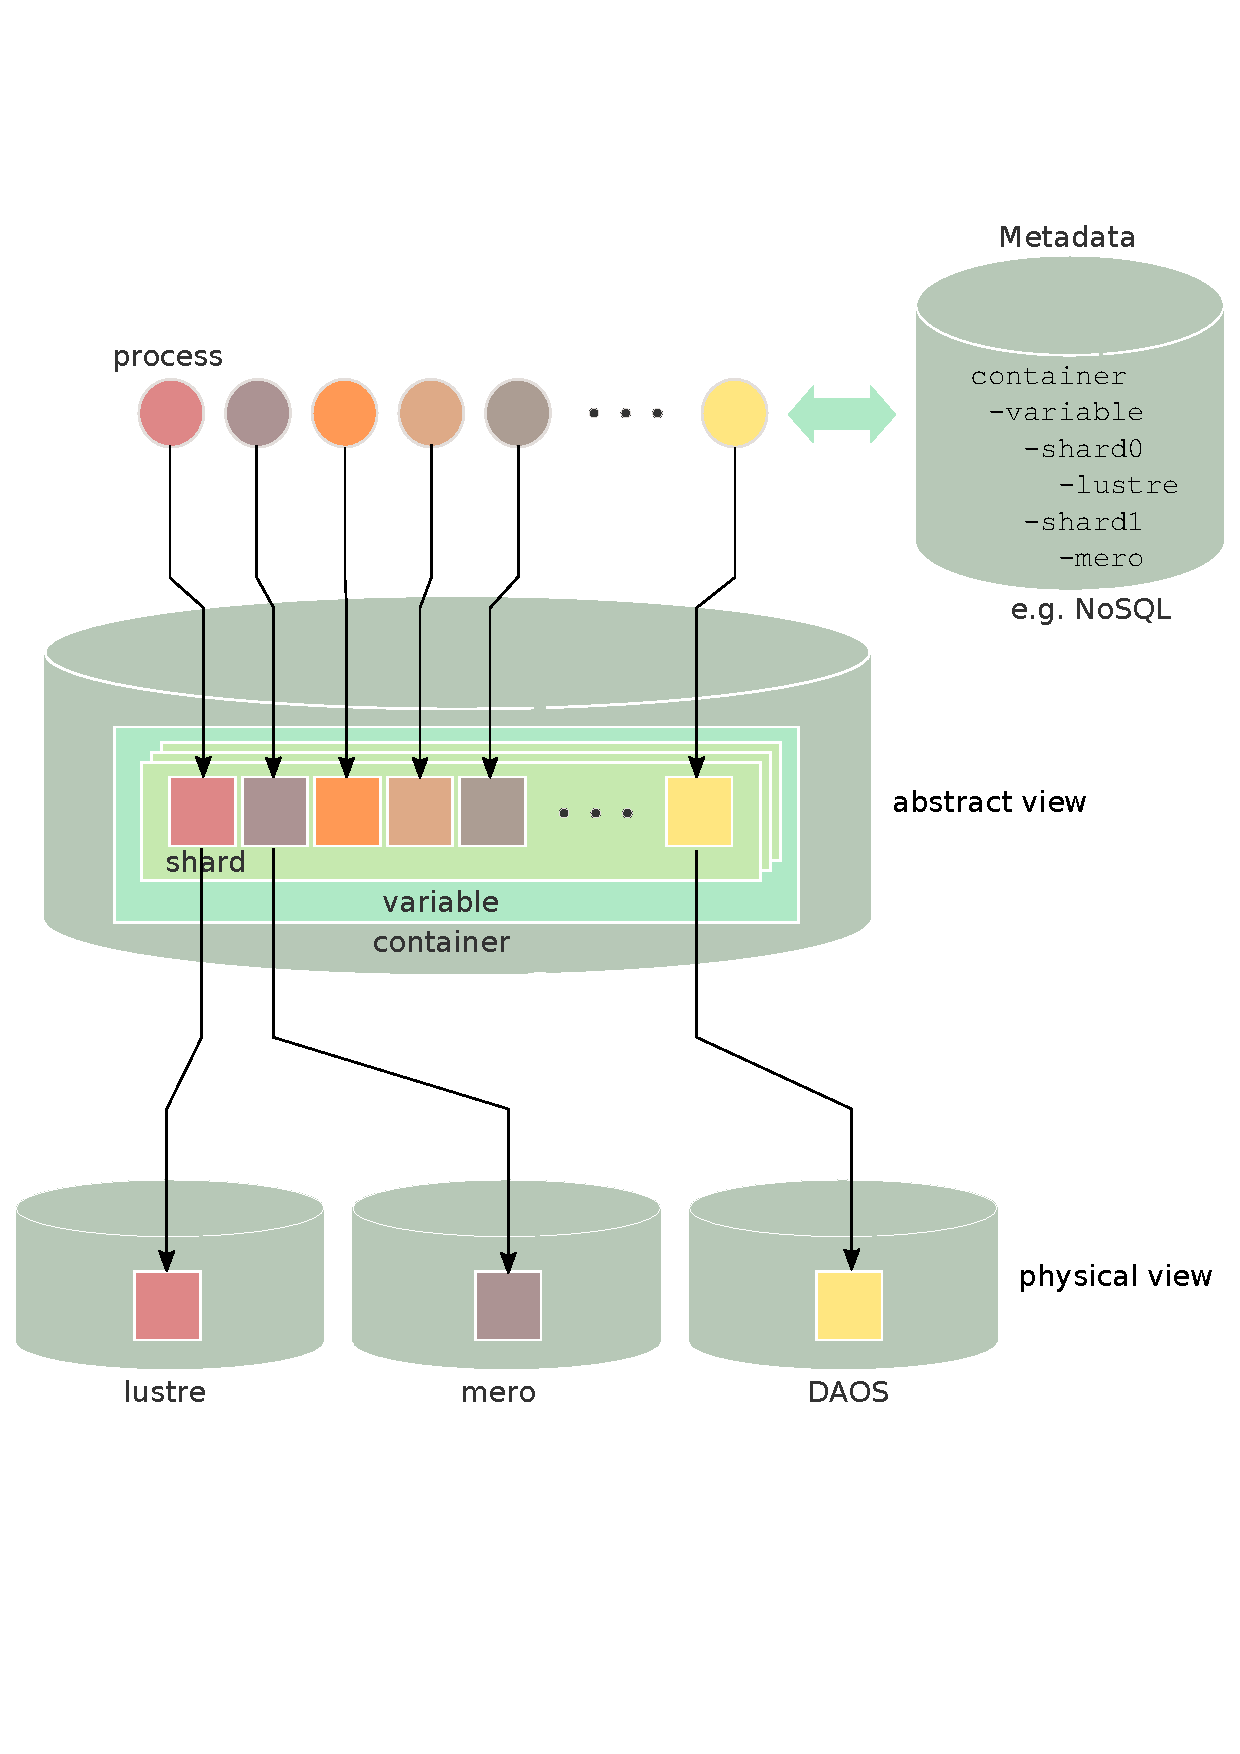
\includegraphics[width=0.5\textwidth]{data-model}
    \caption{Logical Data Model}
    \label{fig:data-model}
\end{figure}

Each of these entities is now described, along with a list of supported operations.

\begin{description}

\item[Variable]

In the logical data model, the variable corresponds directly to a variable in the conceptual data model. Each element of the variable sampled across the dimensions contains data with an associated data type.
Variables are combined with both scientific metadata and technical metadata and are partitioned into fragments, each of which can be stored on one or more storage backends.
A variable definition includes internal information about the domain (bounding box in some coordinate system) and dimensionality (size and shape), while the detailed information about which coordinate variables are needed to span the dimensions and how they are defined is held in the technical metadata.  Similarly, where a variable is itself a coordinate variable, a link to the parent variable for which it is used is contained in the technical metadata.
ESDM will not allow an attempt to delete a variable to succeed while any such references exist (see references).
A crucial part of the variable definition is the list of fragments associated with it, and if possible, how they are organised to span the domain.
Users may choose to submit code pieces that then run within the I/O-path (not part within ESiWACE implementation). This operation covers the typical filter, maps and reduces services of the data flow programming paradigm. Fragments are created by the backend while appending/modifying data to a variable.

\item[Fragment]

A fragment is a piece (subdomain) of a variable. ESDM expects to handle fragments as atomic entities, that is, only one process can \texttt{write} a fragment through ESDM and ESDM will \texttt{write} fragments as atomic entities into storage backends.
The backends are free to partition these fragments further as appropriate, for example, by sharding using chunks.
However, ESDM is free to replicate fragments or subsets of fragments and to choose which backend is appropriate for any given fragment.
This feature allows, for example, ESDM to split a variable into fragments, some of which are stored on a parallel file system, while others are placed into the object storage.

\item[Container]

A container is a virtual entity that provides views on collections of variables and allows multiple different data sets (as defined in the conceptual model) the access to the variables visible to ESDM.  Each container provides a hierarchical namespace holding references to one or multiple variables and their metadata. Variables cannot be deleted while a container references them.  The use of dynamic containers provides support for a more flexible organisation of data than a regular file system semantics. In addition, container efficiently support high-level applications such as Data Reference Syntax\footnote{Taylor et al. (2012): CMIP5 Data Reference Syntax (DRS) and
Controlled Vocabularies.}.
A container provides the ESDM storage abstraction analogous to an external file. Because many scientific metadata conventions are based on semantic structures, which span variables within a file in ways that may be opaque to ESDM without the use of a plugin, the use of a container can indicate to ESDM that these variables are linked even though ESDM does not understand why. Therefore, they cannot be independently deleted.
When entire files in NetCDF format are ingested into ESDM, the importing tool must create a container to ensure such linking properties are not lost.

\item[Metadata]

Metadata can be associated with all the other first class entities (variables, fragments, and containers). Metadata is split into internal ESDM technical metadata and external user-supplied semantic metadata.
Technical metadata covers, for example, permissions, information about data location and timestamps.
A backend will be able to add its own metadata to provide information to manage the data fragments from the storage backend managed by it.
The metadata by itself is treated as a standard ESDM variable that is linked to the variable of choice.
The implementation may embed (simple) metadata into fragments of original data (see reference).

\item[Reference]

A reference is a link among entities and can be used in many places.
References can be embedded based on the real data of these logical objects.
For example, dimensions inside a variable can be references and a container typically uses references to variables.

\end{description}

It is crucial to notice that ESDM does not offer a simple hierarchical namespace for the files.
It provides the primary functions to navigate data, teleportation and orientation, in the following fashion:
queries about semantical data properties (e.g., \texttt{experiment=myExperiment, model=myModel, date=yesterday}) can be performed returning a list of matching files with their respective metadata.
Iterating the list (orientation) is similar to listing a directory in a file system.

Note that this reduces the burden to define a hierarchical namespace for data sharing services based on scientific metadata.
An input/output container for an application can be assembled on the fly by using queries and returning the resulting entities.
As a container provides a hierarchical namespace,
by harnessing this capability, one can search for relevant variables and map them into the local file system tree, accessing these variables as if they would be, for example, NetCDF files.
By offering a FUSE client, this feature also enables backwards compatibility for legacy POSIX applications.

\subsection{Physical Data Model}
\label{chap:components and backends}

\tab
This section discusses the most relevant components and backends.
They are ordered according to their position within the I/O stack from the top (application)
to bottom (backend).

The scheduling component breaks down incoming \texttt{read} and \texttt{write} requests into subsequent requests to create or receive multiple fragments. The scheduler relies on a layout component to create a set of domain filling subrequests.
In most cases, an application will not interface directly with ESDM,
but through a standard frontend such as an HDF5 frontend.
A POSIX backend allows interactions with parallel file systems.
Besides data backends, also pure
metadata backends, such as MongoDB, are possible, allowing the use of existing software stacks that typically
reside in some storage backend.

%Object storage backends for Mero (see Section 6.7) and WOS (see Section 6.8) are discussed.

\begin{description}

\item[Scheduling Component]

The I/O requests handled by ESDM are received via the ESDM interfaces.
In most cases, these requests must collect additional information to identify multiple fragments to fulfil a request.
The ESDM scheduler is responsible for progressing potential operations, coordinating requests, and invoking the appropriate handlers.
In particular, the scheduler will consult the layout component to determine which fragments to create or use and which storage backends to choose.

\item[Layout Component]

The layout component is responsible for finding a mapping to storage that takes into account information that is available through the conceptional and logical views of the data.

\item[NetCDF]

NetCDF4 with Climate Forecast (CF) metadata and GRIB evolved to the de-facto standard
formats for convenient data access for the scientists in the domain of NWP and climate. For
convenient data access, it provides a set of features. For example, metadata can be used to
assign names to variables, set units of measure, label dimensions, and provide other useful
information. The portability allows data movement between different, possibly incompatible
platforms, which simplifies the exchange of data and facilitates communication between scientists.
The ability to grow and shrink datasets, add new datasets and access small data ranges
within datasets simplifies the handling of data a lot. The shared file allows keeping the data
in the same file.

\item[Backend POSIX/Lustre]

Most of today's climate applications \texttt{read} from and \texttt{write} to parallel file systems such as Lustre.
In this situation, a POSIX-like backend inside ESDM can handle \texttt{read} and \texttt{write} requests and organise the ESDM data structures.

\item[Mongo DB]

A prototypical metadata backend is designed using MongoDB. This metadata backend
scales horizontally with the number of servers, provides fault-tolerance, and its document model supports arbitrary schemas.
Each type of object in the data model (container, variable, fragment) becomes a collection with indices on specific fields.
Multikey indices allow indexing array fields such as the references.

\item[Mero Backend]

Mero is an exascale ready object store system developed by Seagate and built from the
ground up to remove the performance limitations typically found in other designs. Unlike
similar storage systems (e.g. Ceph and DAOS), Mero does not rely on any other file system
or raid software to work. Instead, Mero can directly access raw block storage devices and
provide consistency, durability and availability of data through dedicated core components.
Like Ceph Mero provides a key-value store component for small data and metadata and an
object storage for raw data.
The key-value store component in Mero can be used to keep track of containers, corresponding
variables and shard inside them. For example, each container will be represented as
an index in Mero. Every index will have references to all the contained variables. Variables are
also described as indices and will contain variable metadata as well as references to shards.
Shards, in this case, can be stored as different Mero objects or files in other storage backends.

\item[WOS Backend]

The DDN WOS object storage solution represents a storage system architecture
which manages data as objects, automatically storing files in the cloud in a
geographically agnostic manner. Each object is stored with a unique OID that is used to retrieve the
related data, delete them or verify the existence. The logical view for interactions between ESDM and Clovis/Mero is illustrated in Figure 6.28.
To interact with the WOS cluster, DDN provides APIs for C++, JAVA and Python languages and an HTTP Restful interface. In particular operations such as \texttt{put}, \texttt{get}, \texttt{delete},
\texttt{exists}, \texttt{reserve} and \texttt{putOID} are allowed in blocking and non-blocking form.

\end{description}

\section{Documentation}

\tab
This section presents the documentation for ESDM (\Cref{doc:esdm}), ESDM applied to NetCDF (\Cref{doc:esdm-netcdf}), three benchmarks (Section \ref{doc:bench}) and Docker instructions (\Cref{doc:docker}) to run the system in different platforms.

\subsection{ESDM}
\label{doc:esdm}

\tab
The following commands install ESDM in Ubuntu/Debian Systems.

\begin{framed}

\# Download and install Git

\texttt{apt-get install git}

\# Git clone ESDM directory from GitHub

\texttt{git clone https://github.com/ESiWACE/esdm.git}

\end{framed}

\begin{framed}

\# Install required packages

\texttt{sudo apt-get install libglib2.0-dev libjansson4 libjansson-dev}

\# Install required packages

\texttt{sudo apt-get install libtool libtool-bin}

\# Install required packages

\texttt{sudo apt-get install automake cmake doxygen subversion}

\# Install required packages

\texttt{sudo apt-get install mpi-default-bin libblacs-mpi-dev}

\# Install required packages (It may not be necessary.)

\texttt{git clone git://git.sv.gnu.org/m4}

\end{framed}

\begin{framed}

\# Build the project

It may be necessary to edit the file \texttt{prepare.sh} using nano, for instance. Just make sure the path for ESDM directory is correct.

\texttt{cd esdm/deps}

\texttt{./prepare.sh}

\texttt{cd ..}

\texttt{./configure --prefix=\$PWD/install --debug}

\end{framed}

\begin{framed}

\# Run the project

\texttt{cd build}

\texttt{make -j 4 install}

\end{framed}

File \texttt{\_esdm.conf} has the configurations for the backends in ESDM.

\begin{framed}

Path: \texttt{esdm/src/test}

\begin{verbatim}
{
  "esdm":    {
     "backends": [
        {
           "type": "POSIX",
           "id": "p1",
           "target": "./_posix1"
        },
        {
           "type": "POSIX",
           "id": "p2",
           "target": "./_posix2"
        }
     ],
     "metadata": {
     "type": "metadummy",
     "name": "md",
     "target": "./_metadummy"
     }
  }
}
\end{verbatim}

\end{framed}

\subsection{ESDM-NetCDF}
\label{doc:esdm-netcdf}

\tab
The following commands install ESDM for NetCDF in Ubuntu/Debian Systems.

\begin{framed}

\# Git clone ESDM-NetCDF directory from GitHub

\texttt{git clone https://github.com/ESiWACE/esdm-netcdf.git}

\# Enter esdm-netcdf directory

\texttt{cd esdm-netcdf/}

\# Update generated configuration files

\texttt{autoreconf --force}

\end{framed}

\begin{framed}

\# Build the project

It may be necessary to edit the file \texttt{build.sh} using nano, for instance. Just make sure the path for ESDM directory is correct.

\texttt{cd build/}

\texttt{./build.sh}

\end{framed}

\begin{framed}

\# Run the project

\texttt{make -j 4 install}

\end{framed}

Once the system is successfully installed, the following message should appear on the screen.

\begin{framed}

\begin{verbatim}

    +-------------------------------------------------------------+
    | Congratulations! You have successfully installed netCDF!    |
    |                                                             |
    | You can use script "nc-config" to find out the relevant     |
    | compiler options to build your application. Enter           |
    |                                                             |
    |     nc-config --help                                        |
    |                                                             |
    | for additional information.                                 |
    |                                                             |
    | CAUTION:                                                    |
    |                                                             |
    | If you have not already run "make check", then we strongly  |
    | recommend you do so. It does not take very long.            |
    |                                                             |
    | Before using netCDF to store important data, test your      |
    | build with "make check".                                    |
    |                                                             |
    | NetCDF is tested nightly on many platforms at Unidata       |
    | but your platform is probably different in some ways.       |
    |                                                             |
    | If any tests fail, please see the netCDF web site:          |
    | http://www.unidata.ucar.edu/software/netcdf/                |
    |                                                             |
    | NetCDF is developed and maintained at the Unidata Program   |
    | Center. Unidata provides a broad array of data and software |
    | tools for use in geoscience education and research.         |
    | http://www.unidata.ucar.edu                                 |
    +-------------------------------------------------------------+

\end{verbatim}

\end{framed}

File \texttt{\_esdm.conf} has the configurations for the backends in ESDM-NetCDF.

\begin{framed}

Path: {\texttt{esdm-netcdf/libsrcesdm\_test/netcdf-bench}}

\begin{verbatim}
{"esdm":
  {
    "backends": [
      {"type": "POSIX", "id": "tmp", "target": "./_esdm",
        "performance-model" : {"latency" : 0.000001, "throughput" : 500.0},
        "max-threads-per-node" : 0,
        "max-fragment-size" : 104857600,
        "max-global-threads" : 0,
        "accessibility" : "global"
      }
    ],
    "metadata": {"type": "metadummy",
        "name": "md",
        "target": "./_metadummy",
        "accessibility" : "global"}
  }
}
\end{verbatim}

\end{framed}

\subsection{Benchmarks}
\label{doc:bench}

\subsubsection{ReadWrite Benchmark Test}
\label{doc:rw-bench}

\tab
This test uses the ESDM high-level API to write a continuous ND subset of a data set. The source code is hosted on Github and can be found using the following URL:

\begin{center}
\url{https://github.com/ESiWACE/esdm/blob/master/src/test/readwrite-benchmark.c}
\end{center}

\tab

\begin{framed}

\# Go to the directory

\texttt{$\sim$/esiwace/esdm/src/test}

\# Run the readwrite-benchmark file

\texttt{./readwrite-benchmark}

\end{framed}

\begin{framed}

\# Output

\texttt{Write: 0.027s 2992.240 MiB/s size:80 MiB}

\texttt{Read: 0.049s 1645.746 MiB/s size:80 MiB}

\end{framed}

\subsubsection{NetCDF Benchmark}
\label{doc:netcdf-bench}

\begin{framed}

\# Go to the directory

\texttt{$\sim$/esiwace/esdm-netcdf/libsrcesdm\_test/netcdf-bench}

\# Run the \texttt{prepare.sh} script

\texttt{./prepare.sh}

\# Run the test

\texttt{./benchtool -f=esdm://longtest -w -r}

\end{framed}

\begin{framed}

\begin{comment}

\# Output

\begin{verbatim}
                                                                               min                  avg                  max
benchmark:write      Open time                                        0.0012904980         0.0012904980         0.0012904980 secs
benchmark:write      I/O time                                         0.0283091750         0.0283091750         0.0283091750 secs
benchmark:write      Close time                                       0.0000326110         0.0000326110         0.0000326110 secs
benchmark:write      I/O Performance (w/o open/close)              1347.5126941171      1347.5126941171      1347.5126941171 MiB/s
benchmark:write      I/O Performance                               1287.3449996970      1287.3449996970      1287.3449996970 MiB/s

                                                                               min                  avg                  max
benchmark:read       Open time                                        0.0001024170         0.0001024170         0.0001024170 secs
benchmark:read       I/O time                                         0.0671569910         0.0671569910         0.0671569910 secs
benchmark:read       Close time                                       0.0000061120         0.0000061120         0.0000061120 secs
benchmark:read       I/O Performance (w/o open/close)               568.0268292828       568.0268292828       568.0268292828 MiB/s
benchmark:read       I/O Performance                                567.1103510780       567.1103510780       567.1103510780 MiB/s
DEBUG [0]        report.c:362   REPORT_END
\end{verbatim}

\end{comment}

\# Output

\begin{table}[H]
%\begin{adjustbox}{angle=270}
\tiny{
\begin{tabular}{lllll}
                                 &                                           &                 min      &            avg     &            max                         \\
benchmark:write  &    Open time                              &          0.0012904980    &      0.0012904980  &      0.0012904980 secs     \\
benchmark:write  &    I/O time                               &          0.0283091750    &      0.0283091750  &      0.0283091750 secs     \\
benchmark:write  &    Close time                             &          0.0000326110    &      0.0000326110  &      0.0000326110 secs     \\
benchmark:write  &    I/O Performance (w/o open/close)       &       1347.5126941171    &   1347.5126941171  &   1347.5126941171 MiB/s     \\
benchmark:write  &    I/O Performance                        &       1287.3449996970    &   1287.3449996970  &   1287.3449996970 MiB/s     \\
                                 &                                           &                               &                      &                                         \\
                                 &                                           &                 min      &            avg     &            max                         \\
benchmark:read   &    Open time                              &          0.0001024170    &     0.0001024170   &      0.0001024170 secs     \\
benchmark:read   &    I/O time                               &          0.0671569910    &     0.0671569910   &      0.0671569910 secs     \\
benchmark:read   &    Close time                             &          0.0000061120    &     0.0000061120   &      0.0000061120 secs     \\
benchmark:read   &    I/O Performance (w/o open/close)       &        568.0268292828    &   568.0268292828   &    568.0268292828 MiB/s     \\
benchmark:read   &    I/O Performance                        &        567.1103510780    &   567.1103510780   &    567.1103510780 MiB/s     \\
                                 &                                           &                               &                      &                                         \\
DEBUG [0]              &         report.c:362                                                      &                 REPORT\_END           &                                         &                                                    \\
\end{tabular}
}
%\end{adjustbox}
\end{table}

\end{framed}

\subsubsection{ESDM Metadata}

\tab
This test checks the metadata APIs of ESDM. The source code is hosted on Github and can be found using the following URL:

\begin{center}
\url{https://github.com/ESiWACE/esdm/blob/master/src/test/metadata.c}
\end{center}

The test creates a file \texttt{mydataset.md} inside the contatiner \texttt{mycontainer} with the metadata information. An example is:

\begin{framed}

\vspace*{-0.3cm}

\texttt{mydataset.md}

\vspace*{-0.3cm}

\begin{verbatim}
"int":{"type":"j","data":3}
\end{verbatim}

\end{framed}

\subsubsection{ESDM Metadata for NetCDF}

\tab
This test checks the metadata APIs of ESDM with NetCDF format. The source code is hosted on Github and can be found using the following URL:

\begin{center}
\url{https://github.com/ESiWACE/esdm/blob/master/src/test/metadata_nc.c}
\end{center}

The test creates two files, \texttt{mydataset.md} and \texttt{myvariable.md} inside the container \texttt{mycontainer} with metadata information. Examples of these files are:

\begin{framed}

\texttt{mydataset.md}

\vspace*{-0.3cm}

\begin{verbatim}
"":{"type":"b","data":null,"childs":{"tech":{"type":"b","data":null},
"attr":{"type":"b","data":null},"special":{"type":"b","data":null}}}
\end{verbatim}

\end{framed}

\begin{framed}

\texttt{myvariable.md}

\vspace*{-0.3cm}

\begin{verbatim}
"":{"type":"b","data":null,"childs":{"tech":{"type":"b","data":null,
"childs":{"dims":{"type":"q2@g","data":[10,20]},"type":{"type":"c",
"data":"k"}}},"attr":{"type":"b","data":null,"childs":{"history":{
"type":"o","data":"This is some history"},"unit":{"type":"o","data"
:"Celsius"}}},"special":{"type":"b","data":null,"childs":{"vars":{
"type":"q2@o","data":["longitude","latitude"]}}}}}
\end{verbatim}

\end{framed}

\subsection{Docker}
\label{doc:docker}

\tab
Docker is a set of coupled software-as-a-service and platform-as-a-service products that use operating-system-level virtualisation to develop and deliver software in packages called containers. The ESDM architecture was tested Using Docker to simulate Ubuntu 16.04 and Ubuntu 18.04. Installation for Fedora/CentOS/RHEL systems is expected to be completed soon.

A virtual operating system can be initialised with Docker using the command:

\begin{framed}

\texttt{sudo docker run -it <operating system> bash}

\end{framed}

\subsubsection{Ubuntu 16.04 and 18.04}

\tab
Start with the following command to create a container for Ubuntu. Both tested versions have the same behaviour. Therefore, they will be included in just one section.

\begin{framed}

\texttt{sudo docker run -it Ubuntu 16.04 bash}

\texttt{sudo docker run -it Ubuntu 18.04 bash}

\end{framed}

This operating system is now unspoiled. Therefore, additional packages have to be installed to enable ESDM to be tested.

\begin{framed}

\texttt{apt-get update}

\texttt{apt-get install git}

\end{framed}

After this step, the procedures are the same described in Sections \ref{doc:esdm} and \ref{doc:esdm-netcdf}. For self-completeness, they are also included here.

\begin{framed}

ESDM

\texttt{git clone https://github.com/ESiWACE/esdm.git}

\texttt{apt-get install libglib2.0-dev libjansson4 libjansson-dev}

\texttt{apt-get install libtool libtool-bin}

\texttt{apt-get install automake cmake doxygen subversion}

\texttt{apt-get install mpi-default-bin libblacs-mpi-dev}

\texttt{git clone git://git.sv.gnu.org/m4}

\texttt{cd esdm/deps}

\texttt{./prepare.sh}

\texttt{cd ..}

\texttt{./configure --prefix=\$PWD/install --debug}

\texttt{cd build}

\texttt{make -j 4 install}

\end{framed}

\begin{framed}

NetCDF

\# Git clone ESDM-NetCDF directory from GitHub

\texttt{git clone https://github.com/ESiWACE/esdm-netcdf.git}

\# Enter esdm-netcdf directory

\texttt{cd esdm-netcdf/}

\# Update generated configuration files

\texttt{autoreconf --force}

\# Build the project

\texttt{cd build/}

\texttt{./build.sh}

\# Run the project

\texttt{make -j 4 install}

\end{framed}

%Note that when using Docker, the command \texttt{sudo} is not necessary.
